\section{Data Description and Preparation}
\label{sec:data-preparation}

\subsection{Data Description}
\label{sec:data-description}

In this project, the Global Health Observatory (GHO) data repository under the World Health Organization (WHO) dataset \cite{WHO} was selected.  The data from 2000 to 2015 for 193 countries, in total 2938 rows available was selected for statistical analysis. For each country and year 22 fields are stored. The detailed description of the fileds is presented in table \ref{tab:description}. For the analysis, only the year 2014 was selected for use from the original table. There were 183 records available in the restricted table, which seems to be large enough for the scope of this analysis.

\begin{table}
  \centering
  \begin{tabular}{@{}p{0.1\linewidth}  p{0.3\linewidth}p{0.5\linewidth}p{0.1\linewidth}@{}}
    \toprule
      & Column Name     & Description                                                             & type \\
    \midrule 
    1 & Status                 & Developed or Developing status                               & string \\
    2 & Life expectancy   & Life Expectancy in age                                             & float, target variable \\
    3 & Adult Mortality    & Adult Mortality Rates of both sexes (probability of dying between 15 and 60 years per 1000 population) & integer \\
    4 & infant deaths      & Number of Infant Deaths per 1000 population & integer \\
    5 & Alcohol              & Alcohol, recorded per capita (15+) consumption (in litres of pure alcohol) & float \\
    6 & percentage expenditure & Expenditure on health as a percentage of Gross Domestic Product per capita(\%) & float \\
    7 & Hepatitis B & Hepatitis B (HepB) immunization coverage among 1-year-olds (\%) & integer \\
    8 & Measles & number of reported cases per 1000 population & integer \\
    9 & BMI & Average Body Mass Index of entire population & float \\
    10 & under-five deaths & Number of under-five deaths per 1000 population & integer \\
    11 & Polio & Polio (Pol3) immunization coverage among 1-year-olds (\%) & integer \\
    12 & Total expenditure & General government expenditure on health as a percentage of total government expenditure (\%) & float \\
    13 & Diphtheria & Diphtheria tetanus toxoid and pertussis (DTP3) immunization coverage among 1-year-olds (\%) & number \\
    14 & HIV/AIDS & Deaths per 1 000 live births HIV/AIDS (0-4 years) & number \\
    15 & GDP & Gross Domestic Product per capita (in USD) & number \\
    16 & Population & Population of the country & number \\
    17 & thinness 1-19 years & Prevalence of thinness among children and adolescents for Age 10 to 19 (\%) & number \\
    18 & thinness 5-9 years & Prevalence of thinness among children for Age 5 to 9(\%) & number \\
    19 & Income composition of resources & Human Development Index in terms of income composition of resources (index ranging from 0 to 1) & number \\
    20 & Year                     & Year & number \\
    \bottomrule
  \end{tabular}
  \caption{Description of the data set fields}
  \label{tab:description}
\end{table}


As shown in Table 1, most of the regressors in the data set are numerical and can be used in the analysis without modifications. Two regressors are not: Status and Country. The first describes the status of the country and can take two values: ``Developing'' (151 rows) and ``Developed''. This variable was interpreted as a factor. As for the second one, country, was not used in the analysis directly, but, as explained later, was helpful to use other data sources to get the missing values.

\subsection{Missing Data}
\label{sec:missing-data}

In table \ref{tab:missing}, information about the missing data in each column of 2014 year data subset is presented. For almost all of the variables, the number of missing data seems to be reasonable. Unfortunately, for two of them, this was not the case: Population and Gross Domestic Product (GDP). The number of problematic rows in this case was large, so a method to restore the missing values was found.

% latex table generated in R 4.0.3 by xtable 1.8-4 package
% Fri Nov 26 11:47:04 2021
\begin{table}[ht]
\centering
\begin{tabular}{rlrrr}
  \toprule
 & name & Present & Missing & MissingPCT \\ 
  \midrule
6 & Population & 142 &  41 &  22 \\ 
  5 & GDP & 155 &  28 &  15 \\ 
  2 & Hepatitis.B & 173 &  10 &   5 \\ 
  9 & Income.composition.of.resources & 173 &  10 &   5 \\ 
  10 & Schooling & 173 &  10 &   5 \\ 
  3 & BMI & 181 &   2 &   1 \\ 
  4 & Total.expenditure & 181 &   2 &   1 \\ 
  7 & thinness..1.19.years & 181 &   2 &   1 \\ 
  8 & thinness.5.9.years & 181 &   2 &   1 \\ 
  1 & Alcohol & 182 &   1 &   0 \\ 
   \bottomrule
\end{tabular}
\caption{Missing data in 2014 year subset}
\label{tab:missing}
\end{table}

The Population variable was considered first. The WHO table was missing data for the populationt for 49 countries. Cook Islands, Dominica, Marshall Islands, Monaco, Nauru, Niue, Saint Kitts and Nevis, and San Marino were missing one record each; Eritrea had four missing; and 40 other countries (including USA and Great Britain) did not have any information about the population at all.

It iseemed not prudent to exclude such a large amount of data from the analysis, so other source for the missing information was found. The site \cite{WB}, contained the population values for all the years and countries under consideration (in the following it will be referred to as WB table). Some technical work was required to import this information into the WHO data set. A key column had to be massaged into the correct format for the country as the exact spelling of the names of some countries in the two data sets was different. For example, USA in the WHO table was referred to as ``United States of America", while in WB table it was named ``United States", another example is ``United Kingdom of Great Britain and Northern Ireland" vs simple ``United Kingdom".  In total, there were 32 such disagreements.

While comparing the information contained in the population field, it was discoverd that some of the existing data in the WHO dataset did not correspond with the values existing in the WB dataset. A question arose: which data source is more reliable? In figure \ref{fig:afghanistan_pop_comparison} Afghanistan population from two data sets is shown. It became evident that the WHO field for population was error prone. Some years, values of 2 or 3 order of magnitude leaps were found. The WB results, on the other hand, seemed more stable. A determination was made to rely upon the WB population data for all countries under consideration.


\begin{figure}
  \centering
  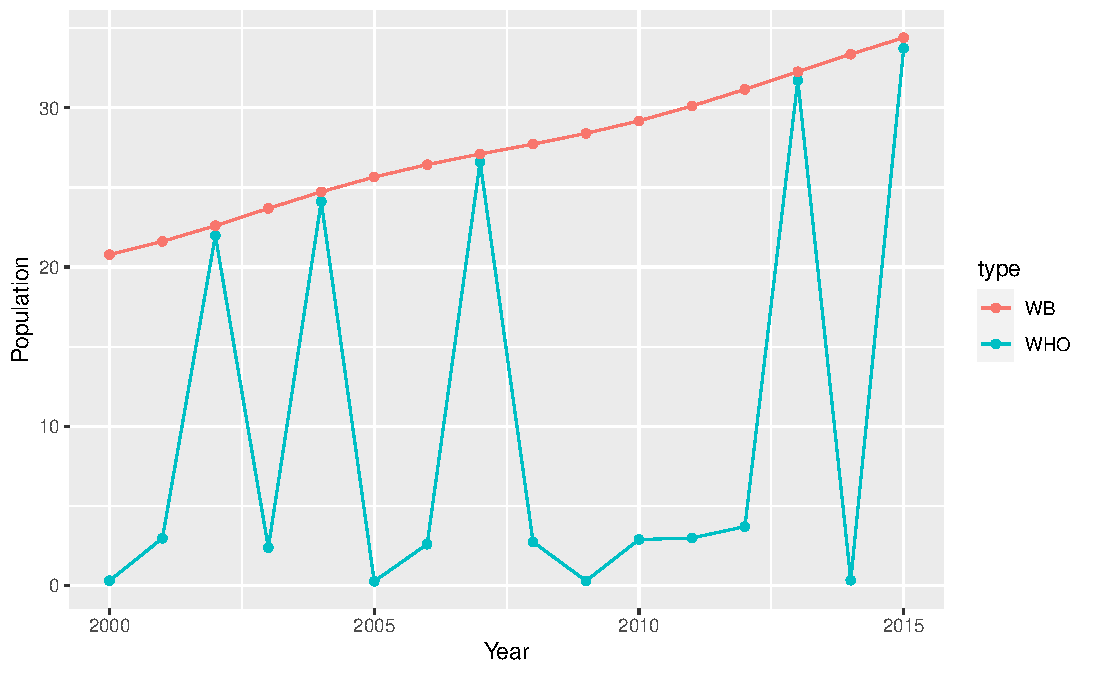
\includegraphics[width = 0.9\textwidth]{figures/Afghanistan_population_comparison}
  \caption{Afghanistan population: comparison of WHO and WB data}
  \label{fig:afghanistan_pop_comparison}
\end{figure}

Almost the same can be said also about the GDP field. The Cook Islands, Monaco, Niue, Papua New Guinea, Saint Kitts and Nevis, San Marino, and Sao Tome and Principe was missing values in one year. Eritrea, Iraq, and Libya were missing four values per each country. South Sudan and Syrian Arab Republic were missing eight values and 26 other countries (including UK) did not have any information at all. As a result, the data table from Global Health Data Exchange (GHDx) database \cite{GHDx} was selected for use for all countries for consistency.

As shown in table \ref{tab:missing}, there were also missing values in some other fields, but not a lot. Since data cleaning was not the main part of this project, a decision was made to simply drop the 26 affected rows.


% \subsection{Variables' Transformation}
% \label{sec:vari-transf}



% ## data description

% ## data cleaning


%%% Local Variables:
%%% TeX-master: "main"
%%% End:
